\documentclass{article}
\usepackage{tikz,amsmath}
\usepackage{comment}
\begin{document}

\noindent\textbf{Q.8.} Use Liebmann's iteration formula to solve Laplace equation
$\dfrac{\partial^2 u}{\partial x^2}+\dfrac{\partial^2 u}{\partial y^2}=0$ at the interior mesh points of the square region with boundary values given in the following figure.

\begin{center}
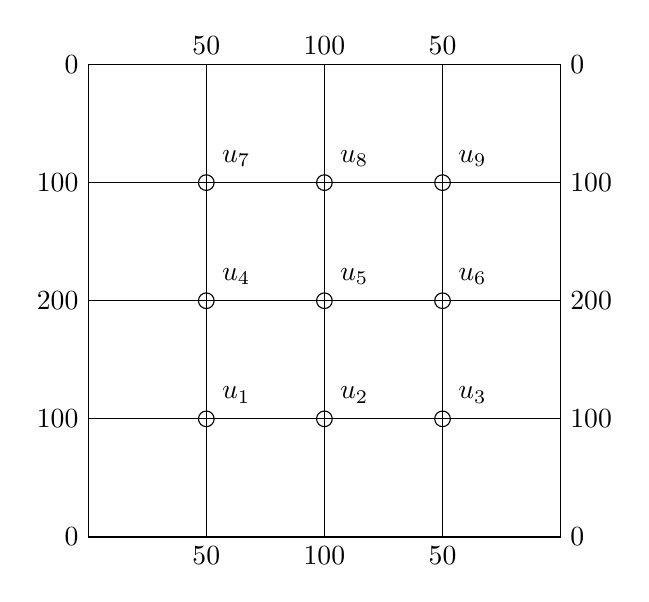
\begin{tikzpicture}[scale=1.5]
\draw (0,0) grid (4,4);
\foreach \n/\x/\y in {1/1/1,2/2/1,3/3/1,4/1/2,5/2/2,6/3/2,7/1/3,8/2/3,9/3/3}
  \node[circle,draw,inner sep=2pt,label={above right:$u_{\n}$}] at (\x,\y) {};
\foreach \v [count=\i] in {50,100,50}{\node[above] at (\i,4) {\v}; \node[below] at (\i,0) {\v};}
\foreach \v [count=\i] in {100,200,100}{\node[left] at (0,\i) {\v}; \node[right] at (4,\i) {\v};}
\node[left] at (0,0) {0}; \node[left] at (0,4) {0};
\node[right] at (4,0) {0}; \node[right] at (4,4) {0};
\end{tikzpicture}
\end{center}

\noindent[Take 2 iterations and obtain the result correct up to three decimal places.]
\begin{comment}
	
	
	multirow provides \multirow{2}{*}{Seasons}, which makes the “Seasons” cell span two rows. The * means the cell takes its natural width.
	array provides the m{width} column type, a fixed-width column whose content is vertically centred. It also provides *{n}{...} for repeating column specs. Many LaTeX distributions load it automatically when tabular is used, but it’s safest to include it.
	
	Commands built into LaTeX (no package needed):
	\multicolumn{5}{|c|}{Sales Data} merges 5 columns into one centred cell, and the | keeps the borders.
	\hline draws a full-width horizontal line.
	\cline{2-5} draws a line only under columns 2 to 5, so it leaves the “Seasons” cell open.
	
	--------------------
\end{comment}
\end{document}
